\begin{figure}[!h] \centering
  \begin{tabular}{cc}
    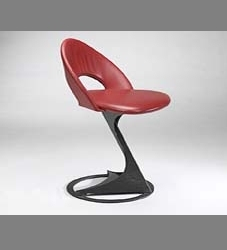
\includegraphics[width=0.45\textwidth]{images/chair_calatrava} &
    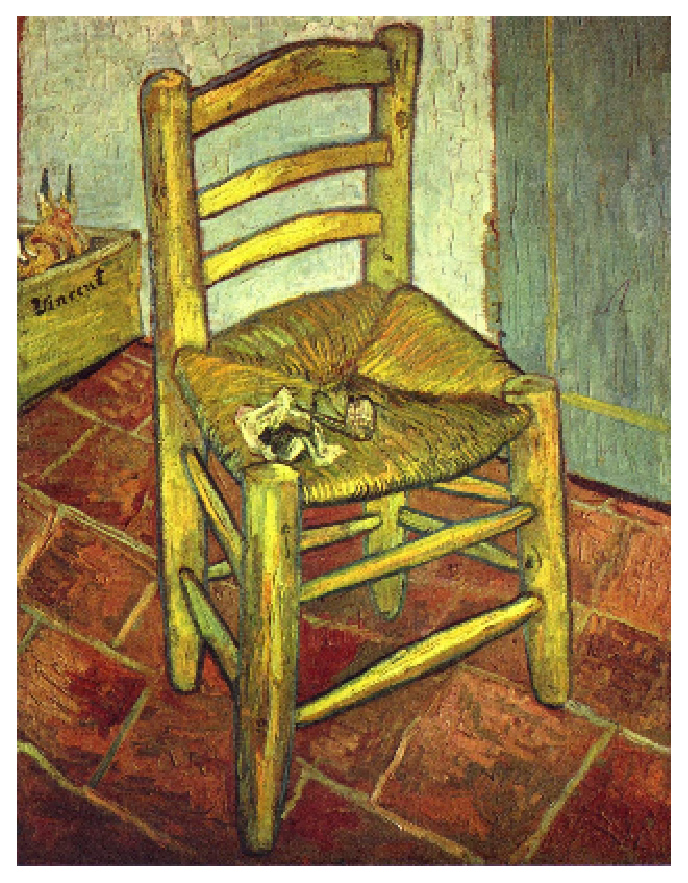
\includegraphics[width=0.45\textwidth]{images/chair_vangogh} \\
  \end{tabular}
  \caption{Two very different chairs: (left) Santiago Calatrava's \emph{Tabourettli}
    (1986) and (right) reproduction from \emph{Vincent's chair} by Vincent Van Gogh
    (1888).}
  \label{fig:chairs}
\end{figure}

Consider Figure \ref{fig:chairs}. What enables us to immediately claim that both
these objects are chairs? The answer is simply: both can be used to sit, and have
been designed to this end. Although nothing in
their visual appearance ties them together, we all know what can be done with such
objects since we have \emph{done} it, at some time in the past. The category of an object
is often determined by its function too, rather than by its visual appearance alone,
and this consideration has led to the re-definition of the concept of ``object''
by Gibson \cite{gibson1,gibson2} in terms of its affordances --- ``what one can do with it''.

The theory of affordances has recently found neurological evidence,
it is claimed, in the mirror neurons paradigm \cite{gallese-96,rizzolatti-04}, according to which
neural correlates exist for both the performance of a grasping
action (mainly involving the sensorimotor system of primates) and its visual
representation when performed by another primate (involving the visual system only,
\cite{umilta-01}). If this is true, then the monkeys' (and our own) object classification is
so robust mainly because these biological systems \emph{know what to do} with the
objects they see --- a capability which machines lack, so far. Picture, for instance,
how much easier automated object recognition of a mug would be under changing illumination
conditions, if only our machine had an idea of how to grasp something which looked like
a mug.

Inspired by these considerations, we hereby define a theoretical framework for
reconstructing \emph{active} sensory modalities from \emph{passive} ones, that is in
short, for figuring out what to do with what one sees, hears, smells etc. In particular,
we enforce one such schema using a multi-variate regression technique to associate
\emph{object visual features} to related \emph{human grasping postures}. This schema is
called a \emph{Visuo-Motor Map} (VMM) and is trained
using a large database of visual and motor data collected from human subjects, that
we call the \emph{Visuo-Motor Grasping dataBase} (VMGdB). The immediate result is the
ability of retrieving a (set of) grasping posture(s) just by seeing an object; this
ability, which we call \emph{grasp priming}, has obvious applications in robotic fields
where (semi)autonomous grasping / fine manipulation is reuquired, such as robotic surgery,
humanoid robotics, teleoperation, advanced hand prosthetics etc. This connection between
robotics and the mirror theory has been explored, although not to this extent, at
least in \cite{lopes-05,metta-06}.

Notice that this problem is, in general, ill-posed, since an object can be grasped in
many distinct ways: a direct inverse mapping from visual to motor features is impossible.
So we resort to a probabilistic estimation: given the sight of an object, how would I
\emph{most likely} grasp it? This solution is similar to that found for motor-based speech
recognition, e.g., in \cite{richmond2007}. More in detail, \textbf{ANNALISA e DISI-jin, volete
approfondire brevemente?}

Lastly, since the focus of this work is on enhancing object reocgnition, we show
that the grasping posture estimation reconstructed by the VMM dramatically improves the
classification rate of a standard object classifier. The visual/motor cue integration is
realised via \textbf{BABI, TATIANA, questo e` vostro}. Our experimental analysis shows
that \textbf{e qui mettiamo i numeri principali dei risultati sperimantali.}

The paper is organised like this: in Section \ref{sec::framework} we define the general
multi-modal learning framework, and then we describe the instance under examination;
we then describe in detail the vision-related unit (Section \ref{sec::vision}) and the
regression schema employed to build the VMM (Section \ref{sec::regression}). We then show our
experimental results (Section \ref{sec::experiments}) and conclude in Section \ref{sec::concl}.

%\begin{itemize}
%
%\item learning by imitation great capability of cognitive systems. It permits to learn how to grasp a cup never seen before just by seeing someone else doing it.
%Fundamental learning mechanism etc 
%
%\item a widely accredited hip is that the underlying mechanism of learning by imitation is the existence of a sensor motor map that links
%the visual perception of an object to the motir position of the hand when it manipulates it. Mirror neurons blabla 
%
%\item another consequence of the existence of a sensor-motor map is that when we learn an object by seeing and manipulating it, we are then able
%to recognize it with a higher degree of accuracy and robustness than if we would have learned it on visual data only. 
%
%\item Enabling a robot to display similar abilities is one of the holy grails of research in artificial cognitive systems. 
%
%\item In this paper we present a mirror neurons inspired algorithm for building perception action maps between visual, passive perception and motor, active
%perception. During learning, the algorithm takes as input visual and sensomotor data and (a) it builds a mapping between the two modalities (b) it builds 
%a classifier on both modalities. After training, wehn presented with a visual input, the system is able to perform grasp priming (= is able to predict
%which are the possible way to grasp the seen object; this information could be used to pre-activate a robot hand) and enhanced visual recognition
%(= is able to recognize objects with a higher degree of accuracy and robustness compared to a model learned only on visual features, even if
%the sensor modality is not perceived by the agent). Experiments show that.....
%
%\item in the rest of the paper...
%
%\end{itemize}
